\section{Boxing / Killing}
\subsection{Singleton}

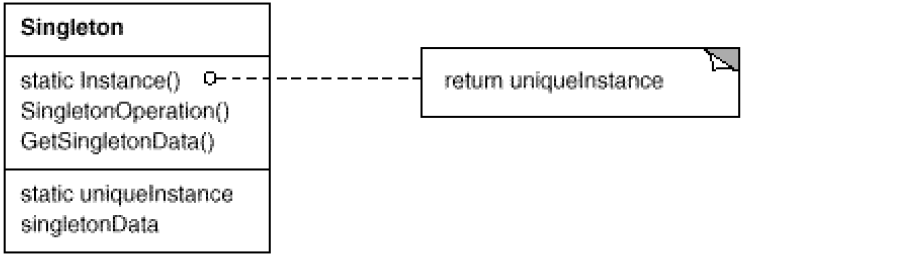
\includegraphics[width=\linewidth]{singleton.png}

\subsubsection{Problem}
\begin{itemize}
    \item Some Classes should have only one instance
    \item The instance must be accessible from a well-known access point
    \item Subclassing from the Singleton should be possible
    \item Extending the Singleton class must not break existing code
    \item How can be guaranteed that only one oject of a class is instantiated and can globally be accessed?
\end{itemize}

\subsubsection{Intention}

\begin{itemize}
    \item Wenn es genau 1 Instanz haben muss
    \item Die Klasse muss global zugreifbar sein
    \item Sub-Klassen einer Singleton-Klasse soll möglich sein
    \item Erweitern der Singleton-Klasse soll Code nicht zerstören
\end{itemize}

\subsubsection{Solution}
Garantiert eine Klasse mit nur einer Instanz. Kann mit einem globalen Punkt auf diesen zuzugreifen \\

\textbf{Solutions inside Singleton}
\begin{itemize}
    \item Singleton Pattern
    \item Class Factory Method
    \item Lazy Acquisition
    \item Eager Acquisition
\end{itemize}
\subsubsection{Consequences}
\textbf{Benefits}
\begin{itemize}
    \item Kontrollierter Zugriffe auf einzige Instanz
    \item Reduziert den Namespace
    \item Erlaubt Verfeinerung von Operationen und Repräsentationen
    \item Erlaubt unterschiedliche Anzahl von Instanzen
    \item Flexibler als Class Operationen
\end{itemize}
\vspace{10pt}
\textbf{Liabilities}
\begin{itemize}
    \item Erstellt eine globale Variable/Zustand
    \begin{itemize}
        \item Clients binden statisch zu einem globalen Klassen Member (enge Kopplung)
        \item Problematisch mit multi-threaded Umgebungen $\rightarrow$ Locking Strategien notwendig
    \end{itemize}
    \item Verhindert Polymorphismus
    \begin{itemize}
        \item Limitiert die Austauschbarkeit
        \item Limitiert Unit Testing (mocking) und verhindert Parallelität während den Tests
        \item Limitiert Application Evolution
    \end{itemize}
    \item Enthält den Zustand bis die Applikation schliesst
\end{itemize}

\vfill\null
\columnbreak

\subsection{Singleton Variation 'Registry'}
\begin{itemize}
    \item More flexible approach
    \item Uses a registry of singletons
    \item Classes registers their singleton in a well-known registry
\end{itemize}
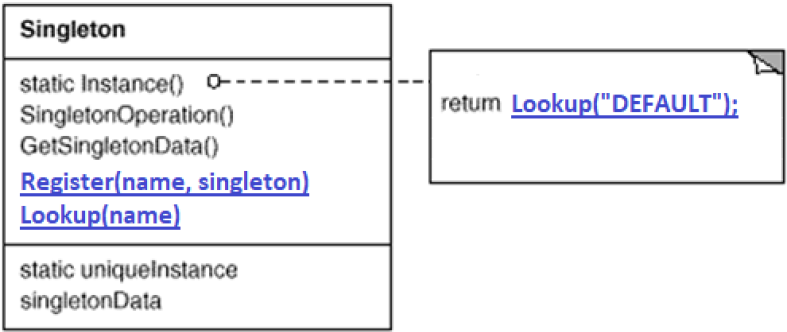
\includegraphics[width=\linewidth]{registry.png}

\subsection{Monostate (Borg) (Killing)}

Mehrere Instanzen sollen das selbe Verhalten haben. Die Instanzen sollen einfach nur andere Namen für das selbe Objekt sein. Sollen sich wie ein Singleton verhalten, ohne dessen Einschränkungen

\subsubsection{Problem}
\begin{itemize}
    \item Multiple instances should have the same behaviour
    \item The instances should be simply different names for the same object
    \item Should have the behaviour of Singleton without imposing the constraint of a single instance
    \item How can two instances behave as though they were a single object?
\end{itemize}

\subsubsection{Solution}

Erstelle ein Monostate-Objekt und implementiere \textcolor{blue}{alle Member} Variablen als statische Members

\begin{lstlisting}
public class Monostate {
    private static int x;
    public int getX() { return x; }
}
\end{lstlisting}

\subsubsection{Consequences}
\textbf{Benefits}
\begin{itemize}
    \item \textcolor{blue}{Transparenz}, man muss nichts über den Monostate wissen
    \item \textcolor{blue}{Derivability} Ableitbar, Sub-Klassen sind erlaubt und teilen die selben statischen Variablen
    \item \textcolor{blue}{Polymorphismus}, verschiedene Ableitungen können unterschiedliches Verhalten haben
    \item well-defined Creation und Destruction
\end{itemize}
\vspace{10pt}
\textbf{Liabilities}
\begin{itemize}
    \item Bricht die Inheritance Hierarchie $\rightarrow$ non-monostate kann nicht zu einem Monostate konvertiert werden
    \item Monostate ist ein echtes Objekt, kann durch viele Creations und Destructions gehen
    \item Monostate statics sind immer alloziert, braucht Speicher
    \item Nicht möglich Monostate-Objekte über mehrere Tier zu sharen
    \item Shared State eines Monostate kann zu unexpected Behavior führen
\end{itemize}

\vfill\null
\columnbreak

\subsection{Service Locator}

Implementierung einer globalen Service-Instanz sollte austauschbar sein. Es soll möglich sein, die Service-Methoden in einem anderen Tier auszuführen.

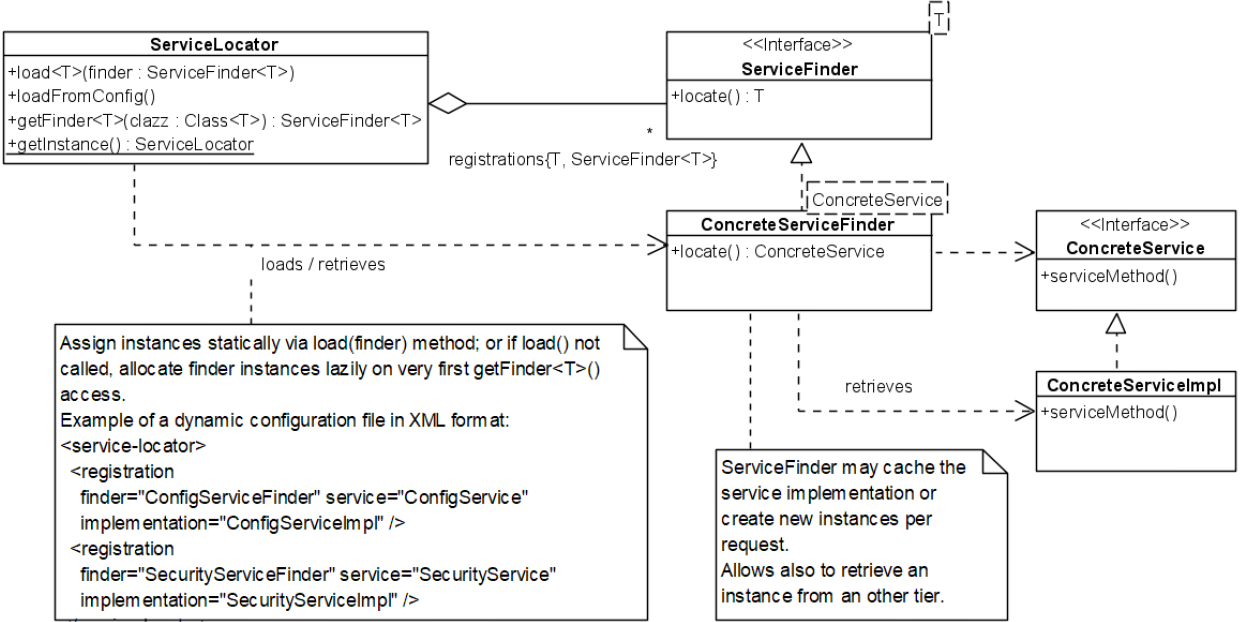
\includegraphics[width=\linewidth]{service_locator.png}

\subsubsection{Problem}
\begin{itemize}
    \item Implementation of a global service instance should be exchangeable
    \item It should be possible to execute the service methods on another tier transparently
    \item How could we register and locate global services when one is needed?
\end{itemize}

\subsubsection{Solution}
Implementierung eines Service-Locators, der weiss, wie man alle Dienste, die eine Anwendung benötigt, findet

\begin{itemize}
    \item Implement the ServiceLocator as a Singleton 'Registry'
    \item ServiceLocator returns \textit{finder} instances, which are used to locate the underlying services
\end{itemize}

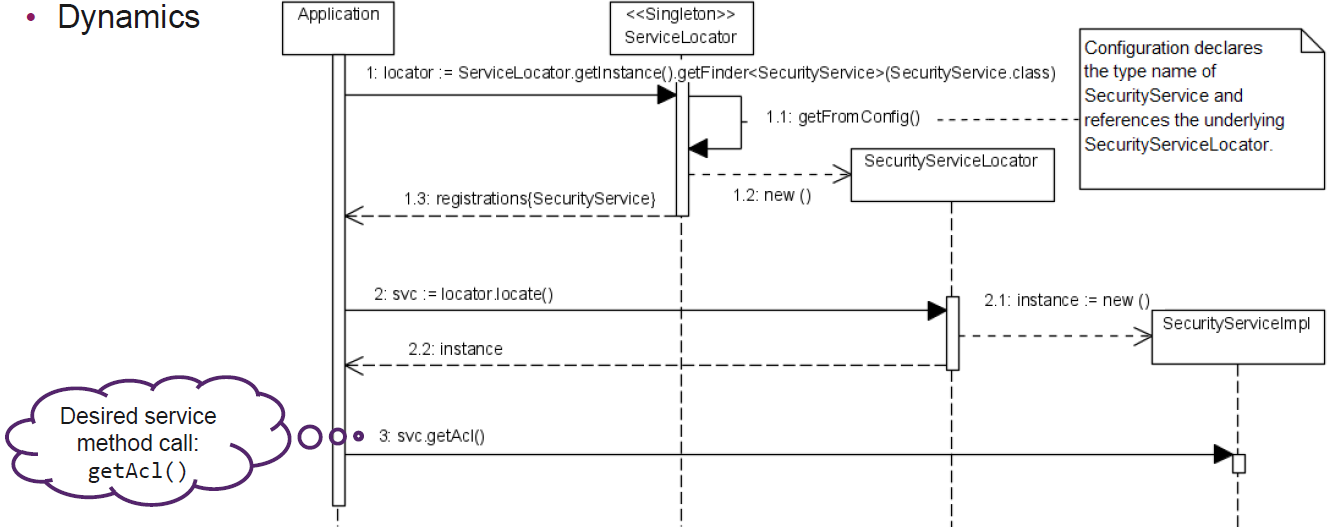
\includegraphics[width=\linewidth]{service_locator_dynamic.png}

\subsubsection{Consequences}
\textbf{Benefits}
\begin{itemize}
    \item Es gibt genau 1 Singleton in der Applikation
    \item ServiceLocator Interface vertraut stark auf Abstraktheit $\rightarrow$ Locators und Services können sogar zur Laufzeit einfach ausgetauscht werden
\end{itemize}
\vspace{10pt}
\textbf{Liabilities}
\begin{itemize}
    \item Clients vertrauten immer noch auf statische Referenzen zum ServiceLocator
    \item Keine Möglichkeit die ServiceLocator Implementation zu ersetzen, aber locators / services sind ersetzbar
    \item Nicht wirklich besser als das Singleton!
\end{itemize}

\vfill\null
\columnbreak

\subsection{Parameterize from Above}

Singleton bietet keine Anforderungen an die Langlebigkeit und die Testbarkeit. Die Applikation wird in einer logischen Art und Weise layered (Horizontal)

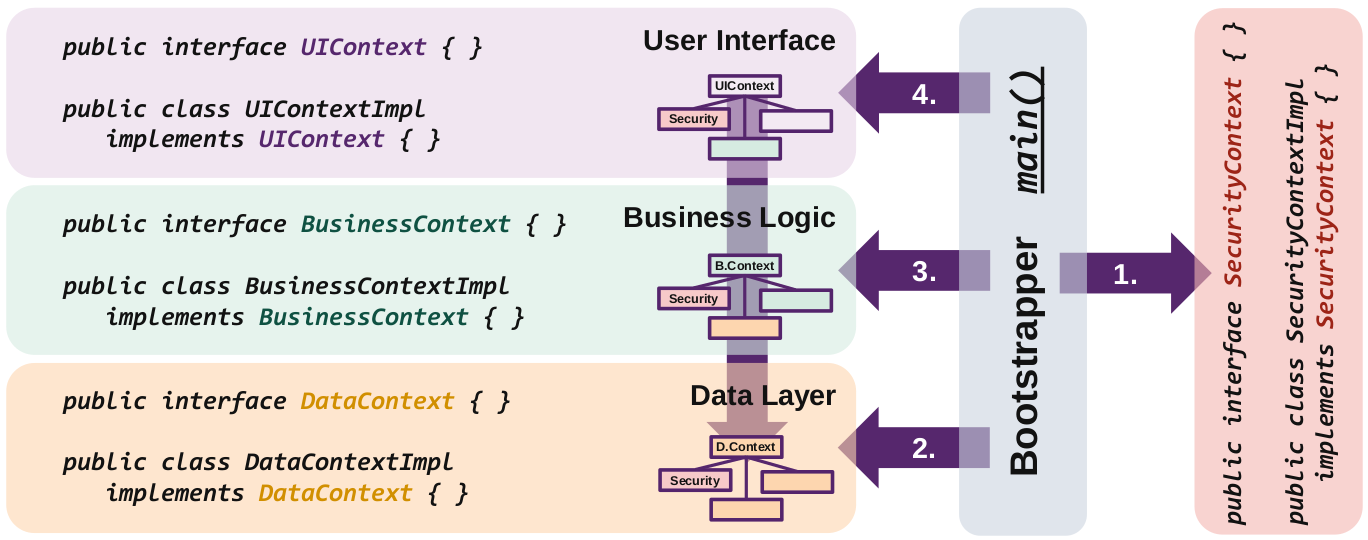
\includegraphics[width=\linewidth]{bootstrapping.png}

\begin{itemize}
    \item Singleton pattern doesn't provide durability and testability requirements
    \item The application has been layered (horizontally) in a logical manner
    \item How can we povide the required application-wide data to the lower layers without making the data globally accessible?
\end{itemize}

\subsubsection{Solution}
Daten die das Verhalten von tieferen Layers beeinflussen sollen von oben überreicht werden

\begin{itemize}
    \item Pass in configuration parameters and 'known' objects rather than having them global
\end{itemize}
\subsubsection{Summary}
\textbf{Benefits}
\begin{itemize}
    \item Keine globalen Variablen
    \item Implementation von parameterisierten Funktionalitäten sind austauschbar
    \item Erzwingt \textcolor{blue}{separation-of-concerns} auf dem Architektur Level
    \item Reduces coupling between layers
\end{itemize}
\vspace{10pt}
\textbf{Liabilities}
\begin{itemize}
    \item Fügt dem Gesamt-System mehr Komplexität hinzu
    \item Kontexte müssen durch den ganzen Applikations-Stack gereicht werden
    \item Fragile Bootstrapper: Applikation muss beim Startup verbunden werden
\end{itemize}

\vfill\null
\columnbreak

\subsection{Dependency Injection}

Benutzer wollen Implementation von existierenden Applikations-Komponenten überschreiben können. Applikation sollte beim Startup verbunden werden.

\subsubsection{Problem}
\begin{itemize}
    \item User may override implementations of existing app components (e.g. test doubles)
    \item Any Componet within the system can demand an object of a specified interface
    \item The Components should not know anything about the wiring mechanism
\end{itemize}

\subsubsection{Solution}

Führe Dependency Injection Container ein, welche die Interfaces und Implementation der Klassen zum Startup lädt und dynamisch instanziert und die Objekte gemäss Dependency Tree verbindet

\begin{itemize}
    \item Central container
    \item Users reference dependencies by the required interfaces
    \item Users apply code annotations
    \item Clients should not address the container directly
\end{itemize}

\subsubsection{Implementation}
\begin{itemize}
    \item Combine \textit{Service Locator} and \textit{PfA}
    \item Container class must not be statically referenced by clients
\end{itemize}
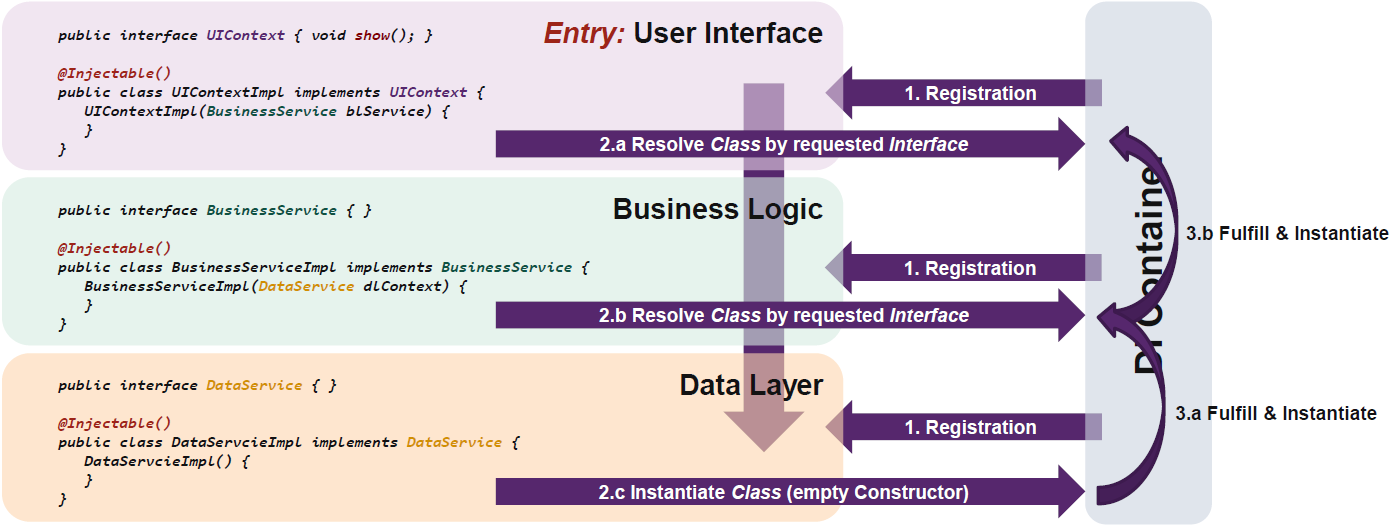
\includegraphics[width=\linewidth]{di_impl.png}

\subsubsection{Consequences}
\textbf{Benefits}
\begin{itemize}
    \item Reduziere die Kopplung zwischen den Consumer und der Implementation
    \item Die Contracts zwischen den Klassen basiert auf Interfaces
    \item Unterstützt das \textcolor{blue}{Open / Closed Principle}
    \item Erlaubt flexibles ersetzen der Implementation
    \item Implementation kann als ''single'' (only on in the system) oder ''transient'' (new instance per injection) markiert werden
\end{itemize}
\vspace{10pt}
\textbf{Liabilities}
\begin{itemize}
    \item Fügt \textcolor{blue}{black magic} dem Gesamt-System hinzu
    \item Den Dependency Tree zu Debuggen kann schwer sein
    \item Rekursive Dependencies sind schwer zu finden und können das Aufstarten des Systems verhindern
    \item Stützt sich auf Reflection und kann zu Performance Verlust führen
\end{itemize}

\vfill\null
\columnbreak

\subsection{Flyweight}

Storage Kosten sind hoch wegen der grossen Menge von Objekten. Viele Objekte können durch relativ wenige gemeinsame Objekte ersetzt werden. Die Objekte sind nicht abhängig von der Objekt-Identität

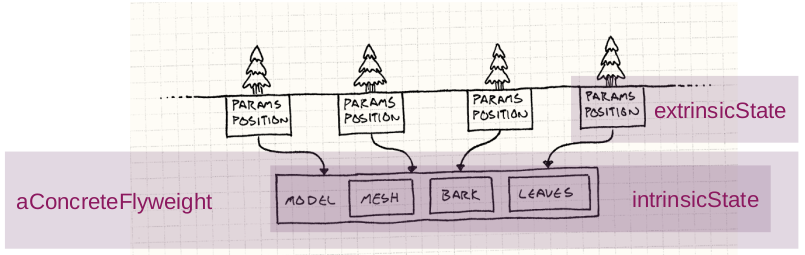
\includegraphics[width=0.8\linewidth]{flyweight-overview.png}

A single pattern for both \textbf{sharing} and \textbf{creation}
\subsubsection{Problem}
\begin{itemize}
    \item Storage costs are high because of the sheer quantity of objects
    \item Many objects bay be replaced by relatively few shared objects
    \item The objects do not depend on object identity
    \item How can multiple copies of a identical constant object be avoided?
\end{itemize}

\subsubsection{Solution}

Verwende Sharing um eine grosse Anzahl von fine-grained Objekte effizient zu unterstützen

\begin{itemize}
    \item Flyweight manager maintains instantiated flyweights
    \item Flyweights must be immutable (readonly)
    \item Context information is often maintained by parent object
\end{itemize}
\vspace{10pt}
\textbf{Use Case}

\begin{enumerate}
    \item Eine Applikation verwendet viele Objekte \\ $\rightarrow$ Shared Objekte sind nicht abhängig von der Identität
    \item Objekt State kann in \textcolor{blue}{intrinsic} und \textcolor{blue}{extrinsic} unterteilt werden \\ $\rightarrow$ Spart Platz, DRY on data
\end{enumerate}

\textbf{Relations}

\begin{itemize}
    \item Oft mit Composite kombiniert
    \item Geht mit fine-graned Elementen um, welche \textcolor{blue}{Immutable Value} Charakteristiken enthalten
    \item Fine-Grained Objekte werden global gespeichert, lazy initialized
    \begin{itemize}
        \item Verhalten ähnlich zu multi-Singleton
        \item Objekte werden in einer Class Factory Ähnlichkeit erstellt
    \end{itemize}
    \item Flyweight enthalten \textcolor{blue}{Pool} von shared Objekten
\end{itemize}

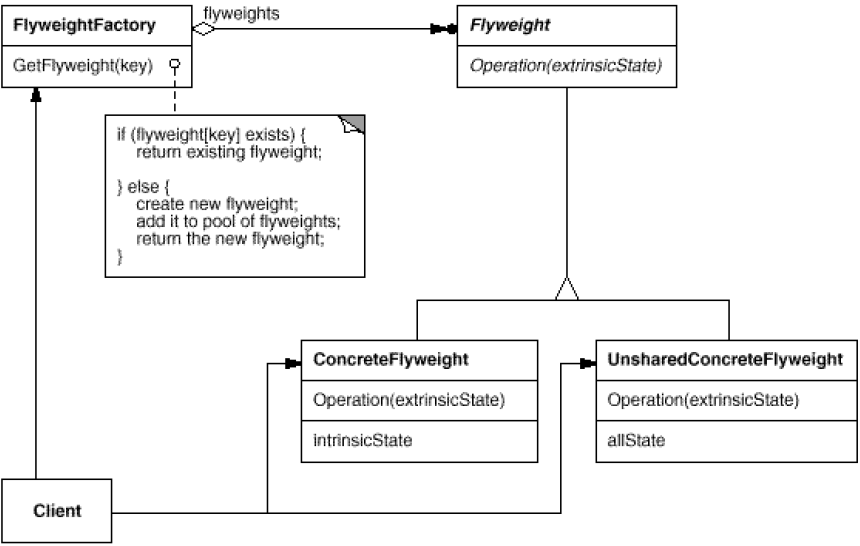
\includegraphics[width=\linewidth]{flyweight.png}
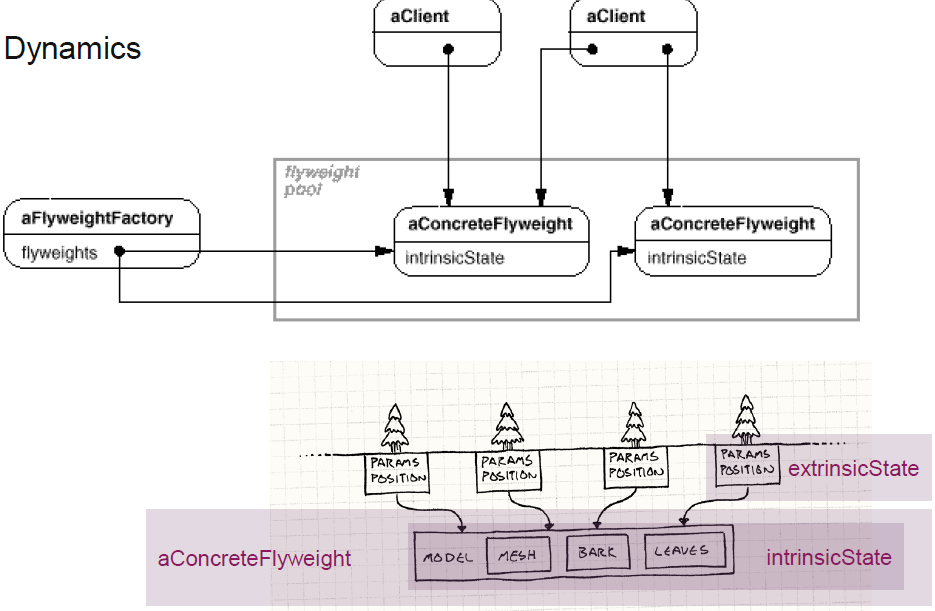
\includegraphics[width=\linewidth]{flyweight_dynamic.png}
\textbf{Solutions inside Flyweight}
\begin{itemize}
    \item Composite
    \item Immutable Value
    \item Pooling
    \item Class Factory Method
    \item Lazy Acquisition
    \item Eager Acquisition
\end{itemize}

\subsubsection{Consequences}
\textbf{Benefits}

Reduktion der gesamt Anzahl von Instanzen. Abhängig von mehreren Faktoren

\begin{itemize}
    \item Reduktion der gesamt Zahl von Instanzen kommt durch das Sharing
    \item Die Anzahl von intrinsic State pro Objekt
    \item Whether extrinsic state is computed (=computation time) or stored(= space cost)
\end{itemize}
\vspace{10pt}
\textbf{Liabilities}
\begin{itemize}
    \item Kann nicht auf Objekt Identität vertrauen. Gespeicherte Elemente enthalten Value Charakteristik
    \item Kann zu run-time Kosten führen. Verbunden mit finden des flyweights und /oder computign extrinsic state
\end{itemize}

\subsection{Pooling (Boxing)}

Ein schneller und predictable Zugriff auf die Ressourcen soll gewährleistet sein. Keine Verschwendung von CPU und Komplexität soll minimal sein.

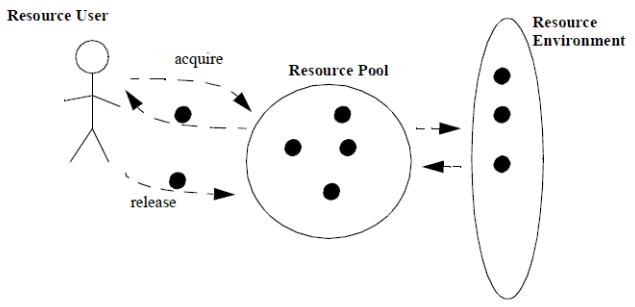
\includegraphics[width=0.7\linewidth]{pooling-2.png}

Beispiel Thread Pool

\subsubsection{Problem}
\begin{itemize}
    \item A fast and predictable access to resources should be provided
    \item Wastage of CPU cycles in repetitious acquisition / release should be avoided
    \item Acquisition / release complexity should be minimized
    \item How can expensive acquisition and release of resources be avoided by recycling resources that are no longer needed?
\end{itemize}
\subsubsection{Solution}
Verwalte mehrere Instanzen eines Types einer Ressource in einem Pool. Dieser Pool von Ressourcen erlaubt Wiederverwendung von bereitgestellten Ressourcen.

\begin{itemize}
    \item A resource pool manages resources and gives them to the users
    \item Resource providers, such as OS, owns and manages the resources
\end{itemize}
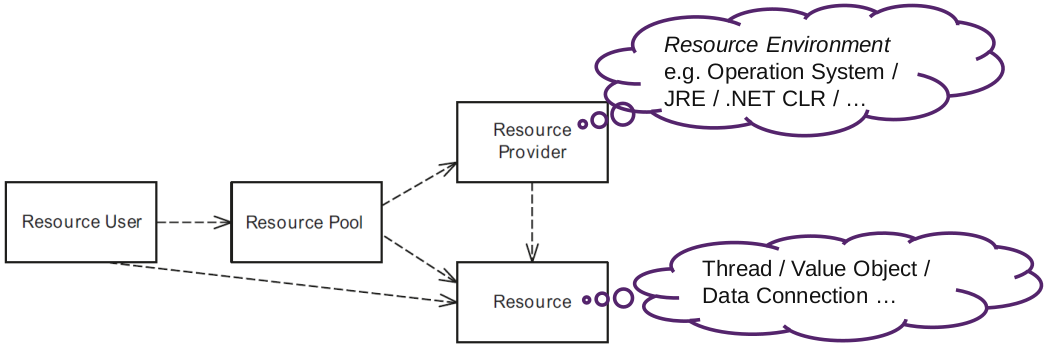
\includegraphics[width=\linewidth]{pooling-1.png}
\subsubsection{Implementation}
\begin{itemize}
    \item Define the maximum number of resources that are maintained by the pool
    \item Decide between \textit{eager} and \textit{lazy} Acquisition
    \item Determine resources recycling/eviction semantics
\end{itemize}

\subsubsection{Consequences}
\textbf{Benefits}
\begin{itemize}
    \item Verbessert die Performanz einer Applikation
    \item Lookup und Release von vorherig-erworbenen Ressourcen ist predictable
    \item Vereinfacht den Release und Erwerb von Ressourcen
    \item Neue Ressourcen können dynamisch erstellt werden
\end{itemize}
\vspace{10pt}
\textbf{Liabilities}
\begin{itemize}
    \item Verwaltete Ressourcen enden in gewissem Overhead
    \item Abhängig von der Umgebung und Ressourcen-Typen, müssen die Ressourcen zu im Pool freigegeben werden
    \item Erwerb-Requests müssen synchronisiert sein um Race Condition zu verhindern
\end{itemize}

\vfill\null
\columnbreak

\subsection{Discussion}
\textbf{Pattern that can be combined with Pooling}
\begin{itemize}
    \item Pool acts as mediator
\end{itemize}
\vspace{10pt}
\textbf{Relation of Flyweight and Pooling}
\begin{itemize}
    \item Flyweight implements a pool with immutable resources statically
\end{itemize}
\vspace{10pt}
\textbf{Is immutability of named resources key?}
\begin{itemize}
    \item No
\end{itemize}
\vspace{10pt}
\textbf{Difference between pooling and caching}
\begin{itemize}
    \item Caching is about handling resources with identity, pooling does not
    \item All resources in a pool are equal
    \item Caching only manages object lifetime in cache, not of objects themselve
\end{itemize}
\vspace{10pt}
\textbf{Patterns in einem Singleton}

\begin{itemize}
    \item Class Factory Method
    \item Lacy Acquisition
    \item Eager Acquisition
\end{itemize}
\vspace{10pt}
\textbf{Benefits for testability with Registry}

Während den Tests kann die Singleton-Instanz mit einem Test-Stub ersetzt werden. Dafür muss der Test-Stub von der Singleton-Instanz erben \\

\textbf{How could you enhance the testability}

Indem das Singleton von einem Basis-Interface ableitet. Dies erlaubt ein komplettes ersetzen innerhalb des Registry \\

\textbf{Application of the Monostate}

In einem sauberen System, soll diese Pattern vermieden werden, aber wenn ein System schon Singleton verwendet können mit dem Monostate die Liabilities mitigiert werden \\

\textbf{Which liability would be most damaging, if Monostate is not documented clearly}

Der \textit{new}-Operator alloziert kein neuen Speicher für das neue Objekt. \\

\textbf{Why does the Monostate-Object break the inheritance hierarchy?}

Ein non-Monostate-Klasse hat einen Internal State (non-static fields). Monostate dürfen dies nicht haben. Somit sind die Hierarchien nicht kompatibel \\

\textbf{What's the relation between Singleton and DI}

\begin{enumerate}
    \item Di Container may implement mechanism to instantiate a requested dependency once per application. Depending on the Di container, such registrations are called
    ''Singleton''.
    \item DI container implementations can be based on the ''Registry'' Singleton variation
\end{enumerate}
\vspace{10pt}
\textbf{What is the improvement of DI over the ServiceLocator Pattern?}

Client classes within the application don't depend directly on the dependency injection container. The DI annotation / attribute allows to reduce the tight coupling between the DI container implementation and the delcarative dependency requirements of a class. Service Locators are directly referenced by client classes. \\

\textbf{What is the defining characteristic of Flyweight?}

Creation, Sharing, use of extrinsic state, immutability and even more... \\

\textbf{Which pattern can be combined with the pooling pattern, if the same resources should be shared between users?}

Pool acts as Mediator $\rightarrow$ Caution consider snychronization when implemmenting Pooling in a multi-threading environment \\

\textbf{What is the relation to the Flyweight pattern and how is it typically implementing the Pooling Pattern?}

Flyweight ist eigentlich ein Pool mit Immutable Ressourcen. Flyweight implements a pool wiht immutable resources in a statically manner. therefore, the flyweight pattern behaves like acombination of singleton and class factory method \\

\textbf{Is immutability of named resources key in the pooling pattern?}

No, it can be implemented as immutable pool of resouces. There are multiple options for pooling resources

\begin{enumerate}
    \item If the items are immutable, the pool is an implementation of the Flyweight pattern
    \item Items can be leased (e.g. Thread Pool), it is an implementation of the Leasing Pattern (POSA 3)
    \item Mutable resouces in Pools can be implemented as prototype Pattern. The consumers recieves not the resource itself but only a clone of them
\end{enumerate}
\vspace{10pt}
\textbf{What is the difference between pooling and caching?}

Pooling wird dann verwendet, wenn die Identität nicht wichtig ist!

\begin{enumerate}
    \item A Pool handles creation, destruction and reuse of the pooled objects
    \item Caching is about managing resources with identity; Pooling does not, all resources in the pool are equal
    \item Caches manage only object lifetime in the cache, but not the lifecycle of the objects themselves.
\end{enumerate}
